% !TeX program = lualatex
% Introduction to Economics for Sport Management -- Lecture 1
% Rebuilt in Beamer from L1.pptx

\documentclass[aspectratio=1610,10pt]{beamer}

% ---------- Engine / fonts ----------
\usepackage{fontspec}
\setmainfont{Calibri}
\usepackage{emoji}
\setemojifont{Segoe UI Emoji}

% ---------- Packages ----------
\usepackage{graphicx}
\usepackage{tikz}
\usepackage{tcolorbox}
\tcbuselibrary{skins}
\usepackage{hyperref}
\usepackage{booktabs}
\usepackage{array}
\usepackage{colortbl}

% ---------- Colours ----------
\definecolor{moldeblue}{RGB}{0,93,163}
\definecolor{moldedark}{RGB}{0,40,74}
\definecolor{accentyellow}{RGB}{255,205,0}

\setbeamercolor{background canvas}{bg=moldeblue}
\setbeamercolor{normal text}{fg=white}
\setbeamercolor{frametitle}{fg=white}
\setbeamercolor{title}{fg=white}
\setbeamercolor{subtitle}{fg=white}
\setbeamercolor{itemize item}{fg=accentyellow}
\setbeamercolor{itemize subitem}{fg=white}
\setbeamercolor{itemize subsubitem}{fg=white}
\setbeamercolor{caption name}{fg=white}
\setbeamertemplate{itemize item}{\textbullet}
\setbeamertemplate{itemize subitem}{--}

\setbeamerfont{frametitle}{size=\Large,series=\bfseries}
\setbeamerfont{title}{size=\LARGE,series=\bfseries}

% ---------- No navigation symbols ----------
\setbeamertemplate{navigation symbols}{}

% ---------- Background: logo (bottom-left) + corner art (bottom-right) ----------
\setbeamertemplate{background}{%
  \begin{tikzpicture}[remember picture,overlay]
    \fill[moldeblue] (current page.south west) rectangle (current page.north east);
    \ifnum\thepage>1
      \node[anchor=south west,inner sep=0pt] at ([xshift=6pt,yshift=6pt]current page.south west)
        {
\includegraphics[height=0.6cm]{images/molde-logo.png}};
      \node[anchor=south east,inner sep=0pt] at (current page.south east)
        {
\includegraphics[height=1.9cm]{images/corner-art.png}};
    \fi
  \end{tikzpicture}%
}

% ---------- Footline: page number + date ----------
\setbeamertemplate{footline}{%
  \ifnum\thepage>1
    \begin{tikzpicture}[remember picture,overlay]
      \node[anchor=south,inner sep=0pt,yshift=6pt] at (current page.south)
        {\footnotesize\color{white!70}\insertframenumber};
      \node[anchor=south west,inner sep=0pt,yshift=6pt,xshift=2.3cm] at (current page.south west)
        {\footnotesize\color{white!70}30 August 2021};
    \end{tikzpicture}%
  \fi
}

\setbeamertemplate{headline}{}
\setlength{\parskip}{6pt}

% ---------- Quote-card environment (rebuilds the George Box "quote card" natively) ----------
\newtcolorbox{quotecard}{
  colback=black, colframe=black, arc=6pt,
  boxrule=0pt, drop shadow, width=0.85\textwidth, halign=center,
  center title, valign=center
}

\title{\Large Introduction to Economics\\ for Sport Management}
\subtitle{Introduction and Preliminaries}
\author{Alessandro Di Mattia}
\date{30 August 2021}

\begin{document}

% ===================== Slide 1 : Title =====================
{
\setbeamertemplate{background}{%
  \begin{tikzpicture}[remember picture,overlay]
    \fill[moldeblue] (current page.south west) rectangle (current page.north east);
    \node[anchor=south west,inner sep=0pt] at ([xshift=6pt,yshift=6pt]current page.south west)
      {
\includegraphics[height=0.6cm]{images/molde-logo.png}};
    \node[anchor=south east,inner sep=0pt] at (current page.south east)
      {
\includegraphics[height=1.9cm]{images/corner-art.png}};
  \end{tikzpicture}%
}
\begin{frame}[plain]
  \vspace{0.3cm}
  \centering
  {\Large\bfseries Introduction to Economics\\[2pt] for Sport Management}\\[10pt]
  {\large Introduction and Preliminaries}\\[14pt]
  {\Large \emoji{soccer-ball}\ \emoji{basketball}\ \emoji{american-football}\ \emoji{tennis}\ \emoji{skis}\ \emoji{video-game}}\\[18pt]
  \begin{columns}[c]
    \column{0.5\textwidth}
      \raggedleft Alessandro Di Mattia
    \column{0.5\textwidth}
      
\includegraphics[height=2.6cm]{images/businessman.png}
  \end{columns}
  \vspace{0.6cm}
  {\footnotesize\color{white!70} 30 August 2021}
\end{frame}
}

% ===================== Slide 2 =====================
\begin{frame}{What is Economics for you?}
  \centering
  
\includegraphics[width=0.55\textwidth]{images/office-brave-face.png}
\end{frame}

% ===================== Slide 3 =====================
\begin{frame}{Economics}
  \begin{itemize}
    \item From Ancient Greek \emph{«oikonomia»}:
    \begin{itemize}
      \item «\emph{oikos}» -- ``family, household''
      \item «\emph{nemein}» -- ``management and dispensation''
      \item Oikos + nemein = «\emph{family/household management}»
    \end{itemize}
    \item Economics as the ``study of wealth'', which studies the process of production, consumption, and accumulation of wealth.
  \end{itemize}
\end{frame}

% ===================== Slide 4 =====================
\begin{frame}{Founders of Economic Thought}
  \centering
  \begin{columns}[T,onlytextwidth]
    \column{0.32\textwidth}
      \centering
      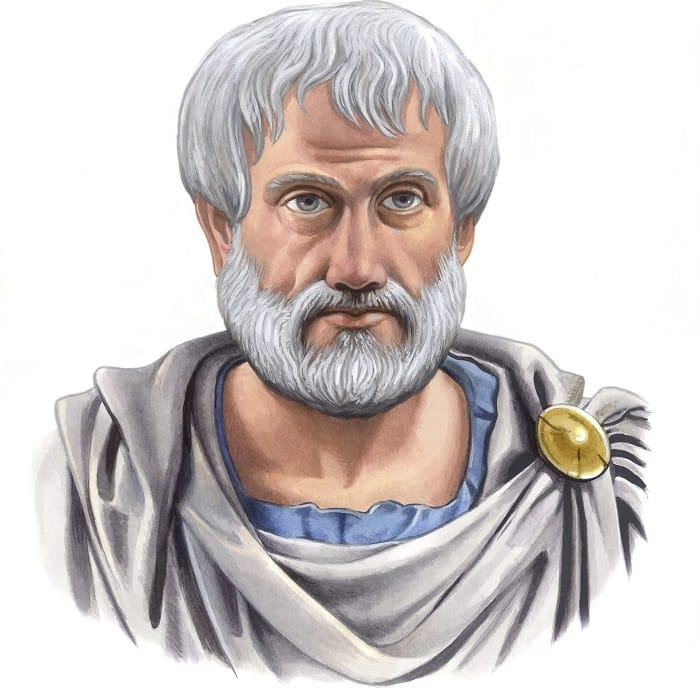
\includegraphics[width=0.85\textwidth]{images/aristotle.png}\\[4pt]
      Aristotle (384--322 BC)
    \column{0.36\textwidth}
      \centering
      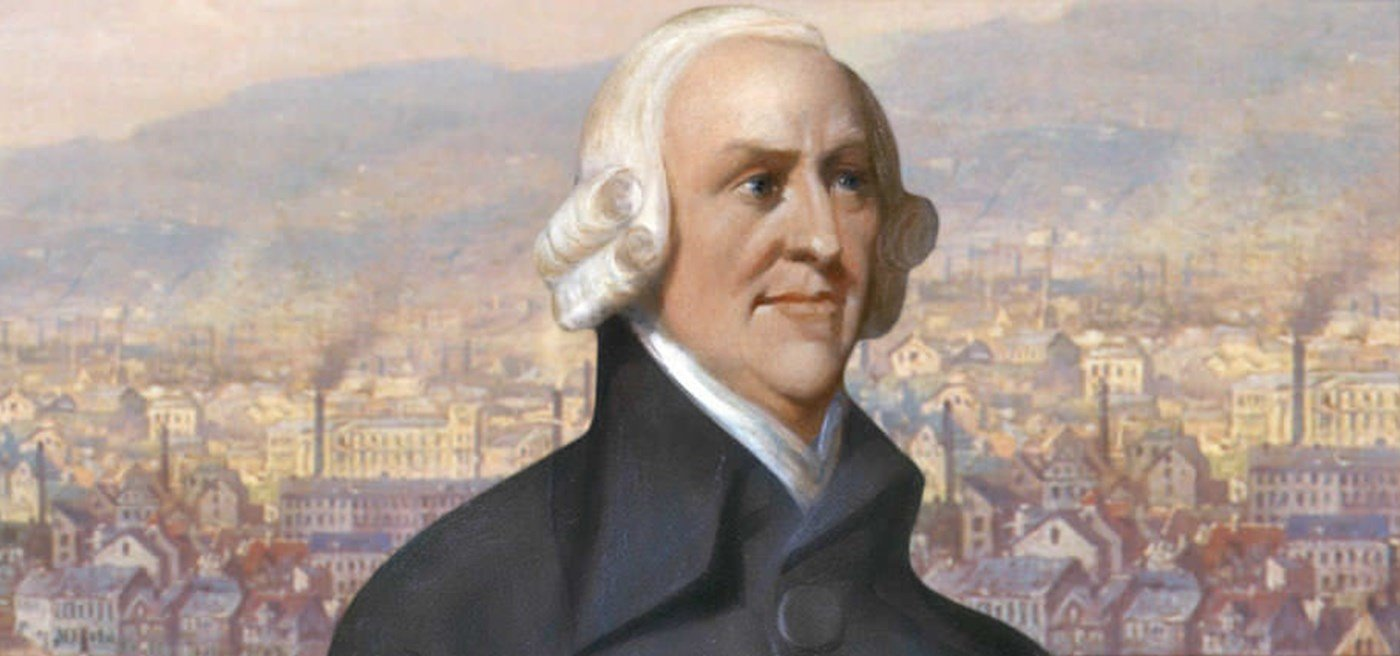
\includegraphics[width=0.95\textwidth]{images/adam-smith.png}\\[4pt]
      Adam Smith (1723--90)
    \column{0.32\textwidth}
      \centering
      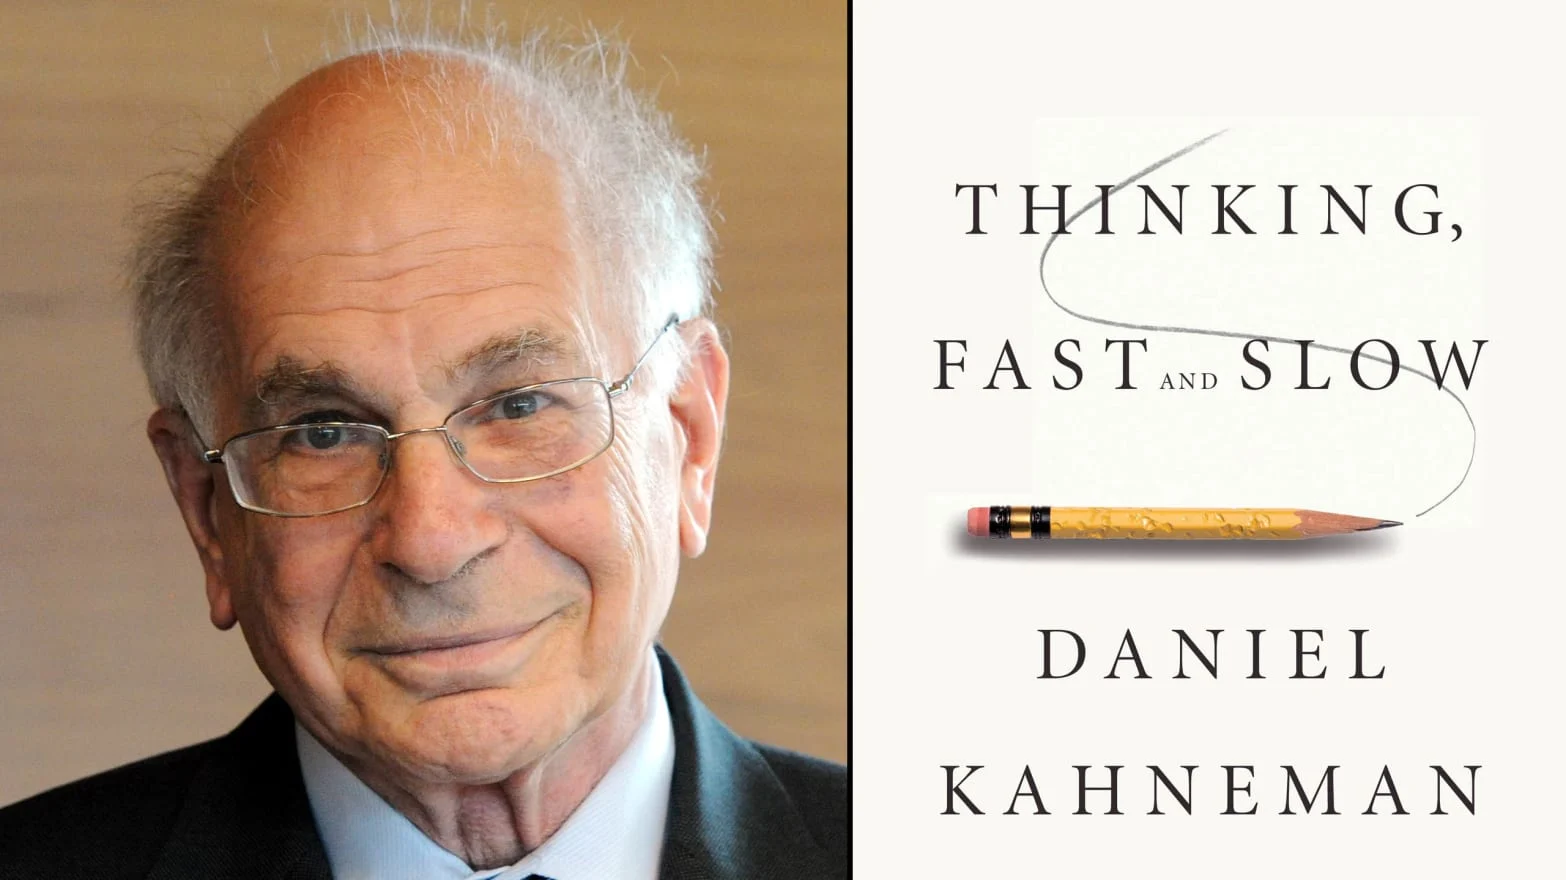
\includegraphics[width=0.95\textwidth]{images/kahneman.png}\\[4pt]
      Daniel Kahneman
  \end{columns}
\end{frame}

% ===================== Slide 5 =====================
\begin{frame}{About the course}
  This is a sophisticated introduction to economics and finance for students like you!

  You will learn:
  \begin{itemize}
    \item The most fundamental tools that economists use
    \item How modern economic theory allows us to understand economic phenomena
  \end{itemize}
\end{frame}

% ===================== Slide 6 =====================
\begin{frame}{Grading Policy}
  \begin{itemize}
    \item Final exam \hfill \textbf{100\%}
    \item Exercises will be posted on Canvas as well as their solutions, after we solve them in class.
  \end{itemize}
  \vspace{6pt}
  \textbf{Prerequisites}
  \begin{itemize}
    \item Basic Algebra and Calculus \emoji{baby}
  \end{itemize}
\end{frame}

% ===================== Slide 7 =====================
\begin{frame}{Course Goals \emoji{key} \emoji{goal-net} \emoji{soccer-ball}}
  Learn main microeconomic concepts and how to use them to analyze real-world problems.

  \textbf{Key Economic Concepts:}
  \begin{itemize}
    \item Marginal Costs and Benefits
    \item Opportunity Costs
    \item Supply and Demand
    \item Value of assets
    \item Interest Rate
  \end{itemize}
\end{frame}

% ===================== Slide 8 =====================
\begin{frame}{Some Important Points}
  \textbf{Advanced course:}
  \begin{itemize}
    \item Use and understanding of formal language, models and math
    \item Interpretation and logic reasoning
    \item Real world implications
  \end{itemize}
  \vspace{6pt}
  Steep learning curve and a toolkit for future course work.
\end{frame}

% ===================== Slide 9 =====================
\begin{frame}{Today: Introduction and Some Basic Concepts}
  \begin{itemize}
    \item Economics as a social science
    \item Methods and fields of study
    \item Basic concepts:
    \begin{itemize}
      \item Normative versus positive analysis
      \item Market Mechanism
    \end{itemize}
  \end{itemize}
\end{frame}

% ===================== Slide 10 =====================
\begin{frame}{Economics: Definition}
  Economics is the study of how a society uses its limited resources to produce, trade and consume goods and services.
  \begin{itemize}
    \item Limited budgets and time for consumers
    \item Limited ability to produce for producers
  \end{itemize}
\end{frame}

% ===================== Slide 11 =====================
\begin{frame}{Economic Imperialism -- A new era?}
  \begin{quote}
  \dots economists have been acting a lot like intellectual imperialists in the last decade or so. They have been using their tools \dots to examine everything from politics to French wine vintages.
  \end{quote}
  \begin{columns}[c]
    \column{0.15\textwidth}
      
\includegraphics[width=\textwidth]{images/nyt-logo.png}
    \column{0.85\textwidth}
      \small ``The Future of Economics Isn't So Dismal'' -- By David Leonhardt, Published: January 10, 2007\\
      \url{https://www.nytimes.com/2007/01/10/business/10leonhardt.html}
  \end{columns}
\end{frame}

% ===================== Slide 12 =====================
\begin{frame}{}
  \centering
  \vspace{0.6cm}
  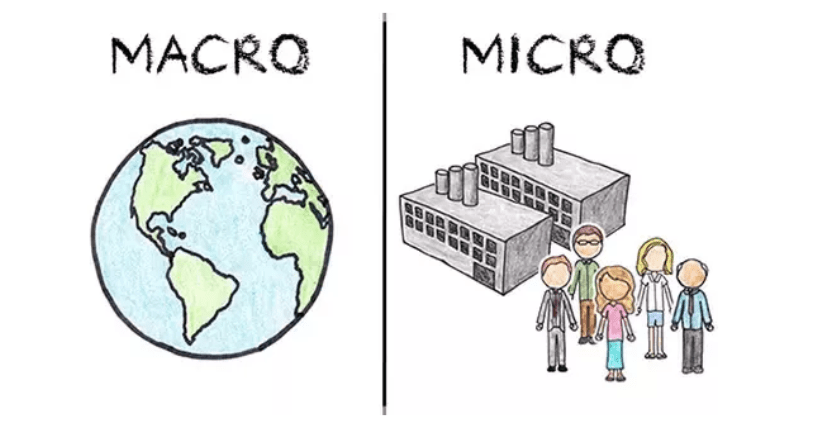
\includegraphics[width=0.7\textwidth]{images/macro-micro-sketch.png}
\end{frame}

% ===================== Slide 13 =====================
\begin{frame}{Microeconomics}
  \begin{itemize}
    \item Study of decisions made by individuals and businesses
    \item Human behavior and decision
    \item Allocation of resources
  \end{itemize}
\end{frame}

% ===================== Slide 14 =====================
\begin{frame}{Themes of Microeconomics}
  \begin{itemize}
    \item Demand, Supply and Equilibrium
    \begin{itemize}\item Prices\end{itemize}
    \item Production theory
    \begin{itemize}\item Creation and manufacture of goods and services\end{itemize}
    \item Cost of production
    \begin{itemize}\item Cost of resources during production\end{itemize}
    \item Labor economics
    \begin{itemize}\item Wages, employment, and income\end{itemize}
  \end{itemize}
\end{frame}

% ===================== Slide 15 =====================
\begin{frame}{Macroeconomics}
  \begin{itemize}
    \item Macroeconomics deals with \underline{aggregate} economic quantities
    \begin{itemize}\item Countries and their policies\end{itemize}
    \item Macro-economist questions
    \begin{itemize}
      \item What should the rate of inflation be?
      \item What causes unemployment?
      \item What are the factors that stimulate or create economic growth?
    \end{itemize}
  \end{itemize}
\end{frame}

% ===================== Slide 16 =====================
\begin{frame}{Microeconomics vs Macroeconomics}
  \small
  \renewcommand{\arraystretch}{1.35}
  \begin{center}
  \begin{tabular}{>{\raggedright\arraybackslash}p{0.44\textwidth}c>{\raggedleft\arraybackslash}p{0.44\textwidth}}
    Analyzes demand and supply of labor & \cellcolor{moldedark}\textcolor{accentyellow}{\textbf{01}} & Analyzes total employment in the economy \\
    Study of decisions made by individuals and businesses & \cellcolor{moldedark}\textcolor{accentyellow}{\textbf{02}} & Study of decisions made by governments in a country \\
    Deals with household and firm decisions & \cellcolor{moldedark}\textcolor{accentyellow}{\textbf{03}} & Deals with performance and behavior of the entire economy \\
    Examines the individual market's behavior & \cellcolor{moldedark}\textcolor{accentyellow}{\textbf{04}} & Analyzes the sum total of the economic activity \\
    Bottom-up approach & \cellcolor{moldedark}\textcolor{accentyellow}{\textbf{05}} & Top-down approach \\
    Investors generally focus in-depth on microeconomics & \cellcolor{moldedark}\textcolor{accentyellow}{\textbf{06}} & Seasoned investors pay little attention to macroeconomics \\
  \end{tabular}
  \end{center}
\end{frame}

% ===================== Slide 17 =====================
\begin{frame}{The Methodology}
  How? Construct \textbf{theories} in order to:
  \begin{itemize}
    \item Understand the different forces driving the economy
    \item Make predictions of what will happen if these forces change
    \item Improve outcomes changing institutions
  \end{itemize}
\end{frame}

% ===================== Slide 18 =====================
\begin{frame}{The Methodology (cont'd)}
  Use \textbf{data} and \textbf{rigorous statistical methods} in order to validate a theory:
  \begin{itemize}
    \item Theories are tested and improved
    \item Theories are invariably imperfect -- but give much insight into observed phenomena
  \end{itemize}
\end{frame}

% ===================== Slide 19 =====================
\begin{frame}{}
  \centering
  \vspace{1.2cm}
  \begin{quotecard}
    {\Large\bfseries\color{white} All models are wrong,\\ but some are useful.}\\[10pt]
    {\small\color{white!80} George Box, British statistician (1919 -- 2013)}
  \end{quotecard}
\end{frame}

% ===================== Slide 20 =====================
\begin{frame}{}
  \centering
  \vspace{0.6cm}
  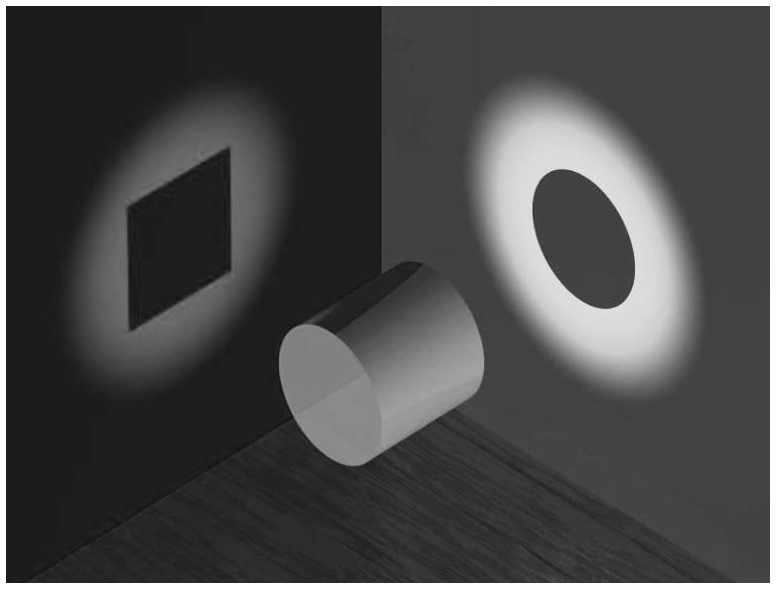
\includegraphics[width=0.62\textwidth]{images/cylinder-shadow.png}
\end{frame}

% ===================== Slide 21 =====================
\begin{frame}{Theories and Models}
  Theories are expressed in the form of \textbf{Economic Models}.
  \begin{itemize}
    \item An economic model is a description of an economic situation via words and mathematical expressions.
    \item Often mathematical expressions are depicted with diagrams.
  \end{itemize}
\end{frame}

% ===================== Slide 22 =====================
\begin{frame}{Economic Models: Description}
  A model usually consists of:
  \begin{itemize}
    \item \textbf{Agents}: their resources, objectives, preferences, how they behave, etc.
    \item \textbf{Economic environment}: markets, contractual arrangements, other relevant institutions.
  \end{itemize}
\end{frame}

% ===================== Slide 23 =====================
\begin{frame}{Positive \& Normative Analysis}
  Economists take different roles: business consultant, media analyst, advisers on government policy, etc.

  It is important to understand when economists are making objective, evidence-based statements (\textbf{positive analysis}) and when they are making value judgements (\textbf{normative analysis}).
\end{frame}

% ===================== Slide 24 =====================
\begin{frame}{Positive Analysis}
  \begin{itemize}
    \item Descriptive and factual statements about the world
    \item Positive does not necessarily mean «good news». Economists can make true negative-positive statements
    \item Positive Analysis uses scientific principles to draw objective and testable conclusions
  \end{itemize}
  \textbf{Examples}
  \begin{itemize}
    \item The unemployment rate is currently at 9\%
    \item Molde FK is winning 1--0 against Viking FK
  \end{itemize}
  \small (Are they negative-positive statements?)
\end{frame}

% ===================== Slide 25 =====================
\begin{frame}{}
  \centering
  \vspace{0.9cm}
  \begin{tikzpicture}
    \clip[rounded corners=18pt] (0,0) rectangle (5.6,3.5);
    \node at (2.8,1.75) {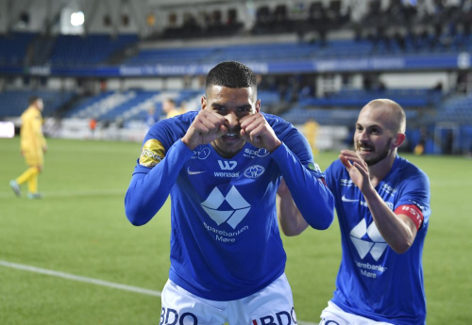
\includegraphics[height=3.5cm]{images/molde-fk.png}};
  \end{tikzpicture}
  \hspace{0.6cm}
  \begin{tikzpicture}
    \clip[rounded corners=18pt] (0,0) rectangle (5.6,3.5);
    \node at (2.8,1.75) {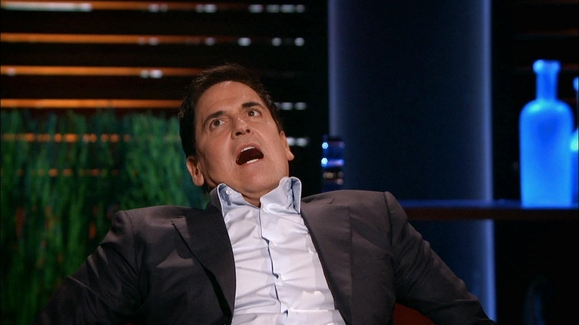
\includegraphics[height=3.5cm]{images/mark-cuban.png}};
  \end{tikzpicture}
\end{frame}

% ===================== Slide 26 =====================
\begin{frame}{Normative Analysis}
  \begin{itemize}
    \item Prescriptive and value-based statements about the world
    \item Normative statements use factual evidence (i.e., positive statements) as support, but they are not by themselves factual
    \item Normative statements incorporate opinions and morals
  \end{itemize}
  \textbf{Examples}
  \begin{itemize}
    \item The unemployment rate is too high
    \item Molde FK is a good team
  \end{itemize}
\end{frame}

% ===================== Slide 27 =====================
\begin{frame}{Causality versus Correlation}
  First, let's watch a video!\\
  \url{https://youtu.be/HUti6vGctQM}

  \vspace{8pt}
  You can find nice examples of spurious correlations, which mean absolutely nothing:\\
  \url{http://tylervigen.com/spurious-correlations}
\end{frame}

% ===================== Slide 28 =====================
\begin{frame}{Required Reading \emoji{orange-book}}
  ``Microeconomics'' edited by Pindyck, Robert S., and Daniel L. Rubinfeld
  \begin{center}
    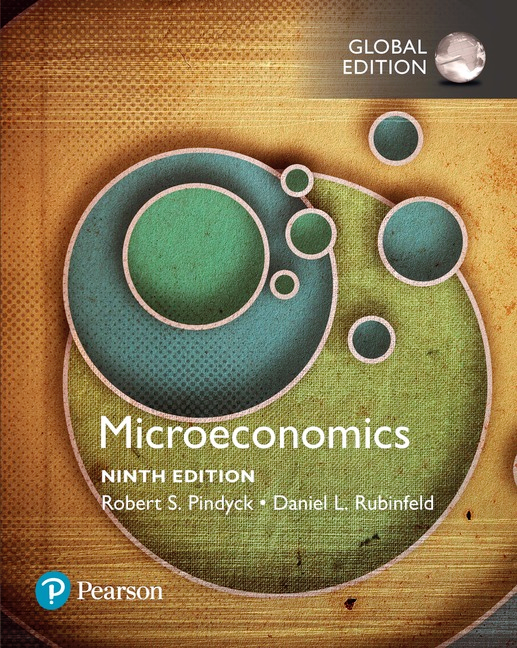
\includegraphics[height=4.6cm]{images/pindyck-cover.png}
  \end{center}
\end{frame}

% ===================== Slide 29 =====================
\begin{frame}{Recommended readings \emoji{books}}
  «Casual Inference: The Mixtape» -- Scott Cunningham\\
  \url{https://mixtape.scunning.com/index.html}
  \begin{center}
    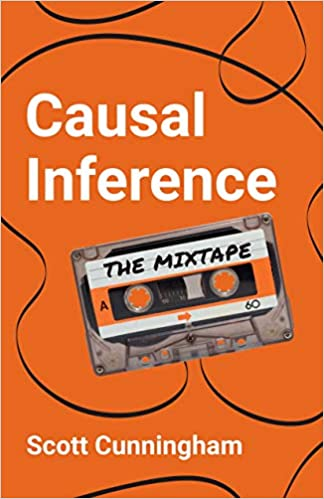
\includegraphics[height=4.6cm]{images/mixtape-cover.png}
  \end{center}
\end{frame}

% ===================== Slide 30 =====================
\begin{frame}{Interesting links}
  \textbf{GDP} \emoji{bar-chart}\\
  \small\url{https://ec.europa.eu/eurostat/statistics-explained/index.php?title=Beginners:GDP_-_What_is_gross_domestic_product_(GDP)}

  \vspace{10pt}
  \normalsize\textbf{Legalizing weed} \emoji{herb}\\
  \small\url{https://www.investopedia.com/articles/insights/110916/economic-benefits-legalizing-weed.asp}
\end{frame}

\end{document}
